\documentclass{uebblatt}

\begin{document}

\maketitle{0}{-- \emph{Spiel und Spaß mit topologischen Basteleien} --}

\begin{aufgabe}{Quotientenräume}
Sei~$X$ ein topologischer Raum und~$\sim$ eine Äquivalenzrelation auf~$X$. Eine
Teilmenge~$U \subseteq X/{\sim}$ soll genau dann \emph{offen} heißen, wenn ihr Urbild
unter der kanonischen Projektionsabbildung~$\pi : X \to X/{\sim}$ in~$X$ offen ist.
\begin{enumerate}
\item Zeige: Diese Setzung definiert eine Topologie auf~$X/{\sim}$.
\item Weise folgende \emph{universelle Eigenschaft} dieser Konstruktion nach:
Sei~$Y$ ein beliebiger topologischer Raum und~$f : X \to Y$ eine stetige
Abbildung. Gelte, dass~$f$ die Äquivalenzrelation auf~$X$ respektiert, d.\,h.
dass äquivalente Punkte gleiche Bilder haben. Zeige, dass es dann genau eine
stetige Abbildung~$\bar f : X/{\sim} \to Y$ gibt, welche das folgende Diagramm
zum Kommutieren bringt.
\[ \xymatrix{
  X \ar[rd]_{\pi} \ar[rrr]^f &&& Y \\
  & X/{\sim} \ar@{-->}[rru]_{\bar f}
} \]
\end{enumerate}
\end{aufgabe}

\begin{aufgabe}{Die reelle projektive Ebene}
Die \emph{reelle projektive Ebene} ist der Quotientenraum~$\PP^2_\RR \defeq
S^2/{\sim}$, wobei~$S^2 \subseteq \RR^3$ die Einheitssphäre ist und die
Äquivalenzrelation genau so definiert wird, dass Antipodenpunkte miteinander
identifiziert werden.
\begin{enumerate}
\item Zeige: Der so definierte Raum ist kompakt und hausdorffsch.
\item Zeige: Die reelle projektive Ebene ist homöomorph zum Ergebnis der
folgenden Bastelanleitung. (Wie ist die Frage formal zu verstehen?)
\begin{center}
  \vspace{0.5em}
  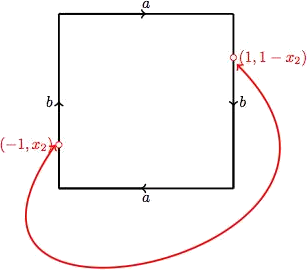
\includegraphics[scale=0.4]{reelle-projektive-ebene}
\end{center}
\end{enumerate}
\end{aufgabe}

\begin{aufgabe}{Triangulierte Räume}
\begin{enumerate}
\item Zeichne Triangulierungen des zweidimensionalen Torus und des Möbiusbands.
\item Wenn du das nicht schon in deiner Kindheit gemacht hast, bastele anschließend
mit echtem Papier ein Möbiusband.
\end{enumerate}
\end{aufgabe}

\end{document}
